\documentclass[UTF8]{ctexart}
\ctexset { section = { format={\Large \bfseries } } }
\pagestyle{plain}
\usepackage{float}
\usepackage{amsmath}
\usepackage{amssymb}
\usepackage{listings}
\usepackage{graphicx}%插入图片宏包
\usepackage{xcolor}
\usepackage{geometry}
\geometry{a4paper,scale=0.8}
\usepackage{caption}
\usepackage{subcaption}
\usepackage[linesnumbered,ruled]{algorithm2e}
\usepackage[colorlinks=true, linkcolor=blue, citecolor=blue, urlcolor=blue]{hyperref}
\captionsetup[figure]{name={Figure}}
\captionsetup[table]{name={Table}}
\definecolor{Rhodamine}{RGB}{227,11,92}

\lstset{
language=Python, % 设置语言
basicstyle=\ttfamily, % 设置字体族
breaklines=true, % 自动换行
keywordstyle=\bfseries\color{blue}, % 设置关键字为粗体,
morekeywords={}, % 设置更多的关键字,用逗号分隔
emph={self}, % 指定强调词,如果有多个,用逗号隔开
emphstyle=\bfseries\color{Rhodamine}, % 强调词样式设置
commentstyle=\color{black!50!white}, % 设置注释样式,斜体,浅灰色
stringstyle=\bfseries\color{red!90!black}, % 设置字符串样式
columns=flexible,
numbers=left, % 显示行号在左边
numbersep=2em, % 设置行号的具体位置
numberstyle=\footnotesize, % 缩小行号
frame=single, % 边框
framesep=1em % 设置代码与边框的距离
}

\title{\textbf{Data Structure lab7}}
\author{吴嘉骜 21307130203}
\date{\today}

\begin{document}

\maketitle

\noindent
\textbf {\large Objective}\\  The objective of this lab is to understand graph representation, sort and search.\\
\noindent
\textbf {\large Experiment environment} \\
   Windows 11 VsCode Python 3.11.5 64-bit\\

\setlength{\parindent}{0pt}
\section*{Problem 1}
Write code for the topological sort of a directed acyclic graph (recursive version).

\textbf{\large Solution}:\\
The code from \texttt{toposort.py} is as follows:

\begin{lstlisting}
def toposort(graph):
    """
    Parameters:
        - graph: a dictionary representing a graph
        
    Returns:
        - a list of vertices in topological order
    """
    def dfs(v):
        # depth first search from vertex v
        visited.add(v)
        for u in graph[v]:
            if u not in visited:
                dfs(u)
        result.append(v)
    
    visited = set()  # visited vertices
    result = []  # topological order of vertices
    
    for v in graph:
        if v not in visited:
            dfs(v)
            
    return result[::-1]  # reverse order
\end{lstlisting}
\textbf{\large Code Interpretation}:\\
For a recursive version of topological sort, we first define a \texttt{dfs} function to perform a DFS starting from a given vertex \texttt{v}. 
It marks \texttt{v} as visited and then recursively calls \texttt{dfs} for all unvisited vertices adjacent to \texttt{v}.
If duplicate vertices are encountered during the recursion, we prune the following search.
After exploring all the adjacent vertices, \texttt{v} is added to the \texttt{result} list. 
This ensures that a vertex is only added after all vertices dependent on it (i.e., vertices that can be reached from it) are added.
Then we call \texttt{dfs} for all vertices in the graph.
Thus, we only need to reverse the result list to get the topological order.

The complexity of this algorithm is \(O(V + E)\), where \(V\) is the number of vertices and \(E\) is the number of edges in the graph. 
This is because each vertex is visited exactly once, and for each vertex, we visit all its adjacent vertices once.

\textbf{\large Test}:\\
We test the code with the following graph of course dependencies, and show one possible result in topological order:

\begin{figure}[htbp]
    \centering
    \begin{subfigure}{0.5\textwidth}
        \centering
        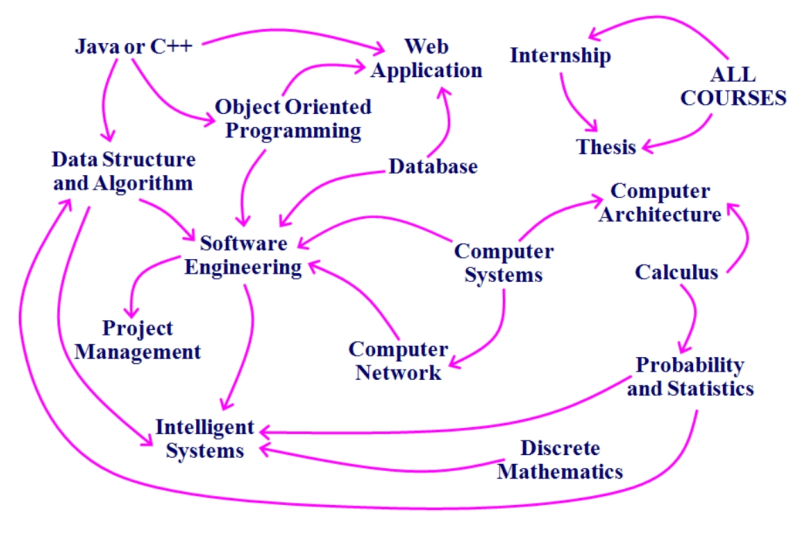
\includegraphics[width=0.8\linewidth]{course.png}
        \caption{Course Dependencies}
    \end{subfigure}%
    \hfill
    \begin{subfigure}{0.5\textwidth}
        \centering
        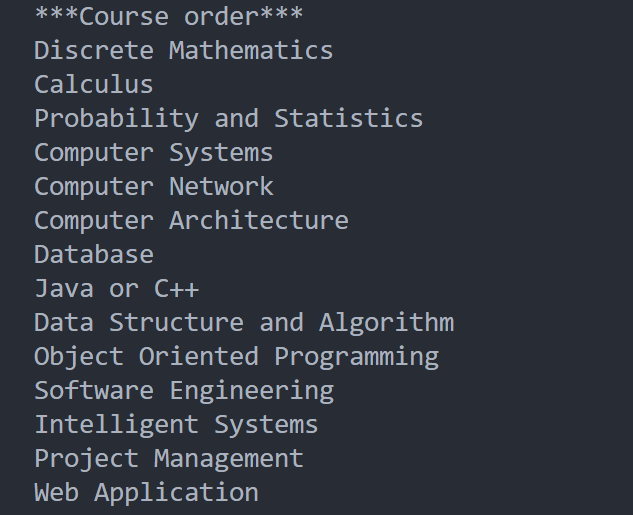
\includegraphics[width=0.7\linewidth]{courseorder.png}
        \caption{Topological Order}
    \end{subfigure}%
    \caption{Course Dependencies and Topological Sort}
\end{figure}

\section*{Problem 2}
Write code (using stack) to solve the following problem. Your implementation needs to print all solution of the problem.\\
\textbf{\large Problem:}\\
A farmer with its wolf, goat, and cabbage come to the edge of a river they wish to cross.
There is a boat at the river`s edge, but, of course, only the farmer can row. the boat also can carry only two things (including the rower) at a time. 
If the wolf is ever left alone with the goat, the wolf will eat the goat;
similarly, if the goat is left alone with the cabbage, the goat will eat the cabbage.
Devise a sequence of crossings of the river so that all four characters arrive safely on the other side of the river.

\textbf{\large Solution}:\\
The code from \texttt{farmerrow.py} is as follows:
\begin{lstlisting}
class State:
    '''
    This class represents a state in the Farmer, Wolf, Goat, and Cabbage.
    '''
    def __init__(self, farmer, wolf, goat, cabbage):
        # Use 1 to represent the start side and 0 to represent the end side.
        self.farmer = farmer
        self.wolf = wolf
        self.goat = goat
        self.cabbage = cabbage
        
    def is_valid(self):
        # Check if the state is valid.
        if (self.wolf == self.goat and self.farmer != self.wolf) or \
            (self.goat == self.cabbage and self.farmer != self.goat):
            return False
        else:
            return True
        
    def is_goal(self):
        # Check if the state is the goal state.
        if (self.farmer == 0 and self.wolf == 0 and self.goat == 0 and self.cabbage == 0):
            return True
        else:
            return False
    
    def __str__(self):
        # String representation of the state.
        return "Farmer: " + str(self.farmer) + " Wolf: " + str(self.wolf) + \
            " Goat: " + str(self.goat) + " Cabbage: " + str(self.cabbage)
        
    def next_state(self):
        # Generate all possibel next states from the current state.
        next_states = []
        items = [self.wolf, self.goat, self.cabbage]
        
        for i, item in enumerate(items):
            if item == self.farmer:  # The item is on the same side as the farmer, so it can be moved.
                next_state = State(1 - self.farmer, *[(1 - self.farmer) if j == i else x for j, x in enumerate(items)])
                if next_state.is_valid():
                    next_states.append(next_state)
        # The farmer can also move alone.
        farmer_alone = State(1 - self.farmer, self.wolf, self.goat, self.cabbage)
        if farmer_alone.is_valid():
            next_states.append(farmer_alone)
        return next_states
    
def cross_river():
    start = State(1, 1, 1, 1)  # Start from the state where all items are on the start side.
    stack = [(start, [str(start)])]  # Use a stack to store the states and the path to the state.
    solutions = []  # Store all solutions.
    
    while stack:
        state_cur, path_cur = stack.pop()
        if state_cur.is_goal():  # Check if the current state is the goal state.
            solutions.append(path_cur)
            continue
        
        for state_next in state_cur.next_state():
            # Check if the next state is already in the path
            if str(state_next) not in path_cur:
                stack.append((state_next, path_cur + [str(state_next)]))
    return solutions

solutions = cross_river()
if solutions:
    print(f"Number of solutions found: {len(solutions)}")
    for i, solution in enumerate(solutions, start=1):
        print(f"\nSolution {i}:")
        for j in solution:
            print(j)
else:
    print("No solution found.")
\end{lstlisting}
\textbf{\large Code Interpretation}:\\
The main idea of this code is to use a depth-first search (DFS) approach to explore all possible states
and find a sequence of actions leading to the goal.

We first define a \texttt{State} class to represent a state specified in this problem.
It initializes the state with the positions of the farmer, wolf, goat, and cabbage as $(1,1,1,1)$, where 1 represents the start side and 0 represents the end side.

The \texttt{is\_valid} method checks if the state is valid, i.e., the wolf will not eat the goat and the goat will not eat the cabbage.
And the \texttt{is\_goal} method checks if the state is the goal state, i.e., all items are on the end side.
To check state redundancy and diaplay the path later, we override the \texttt{\_\_str\_\_} method to return a string representation of the state.

Then we define a \texttt{next\_state} method to generate all possible next states from the current state.
Note that only one item can be moved at a time, and the farmer can also move alone. Considering all possible cases, we still have to check
whether the next state is valid before we add it to the list of next states.

Finally, we define a \texttt{cross\_river} method to perform a DFS starting from the start state. We use a stack to store the states and the path to the state.
If the current state is the goal state, we add the path to the list of solutions. Otherwise, we generate all possible next states and add them to the stack.
FILO property of the stack ensures that we always explore the deepest state first.

I am encountered with a problem when I first wrote the code. I used a set to store the states that have been visited to avoid the same state being visited twice.
The fact is that there may be multiple solutions to this problem, and the same state may appear in different solutions. But we still have to check duplicate states in the same path to avoid infinite loops.
Therefore, I use a list to store the path to the state, and check if the next state is already in the path before adding both the state and path to the stack. This ensures that the same state will not be visited twice in the same path,
while allowing the same state to appear in different paths.

\textbf{\large Result}:\\
The code outputs the following solutions:
\begin{figure}[htbp]
    \centering
    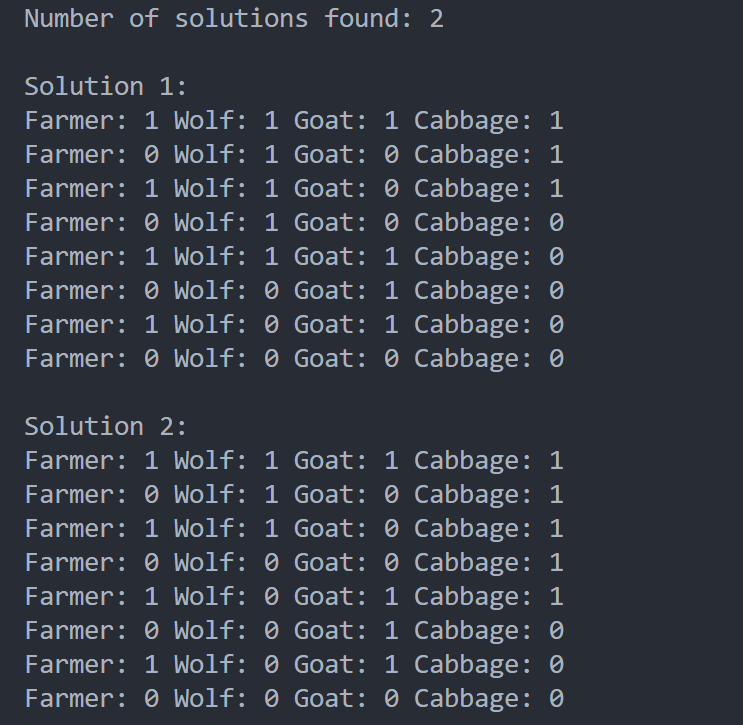
\includegraphics[width=0.45\linewidth]{farmerrow.png}
    \caption{Solutions to the Farmer, Wolf, Goat, and Cabbage Problem}
\end{figure}


\end{document}